\chapter{Évolution Différentielle sur les circuits simple et double diodes}

\section{Introduction}
Maintenant que nous avons abordé les modèles à diodes et l'Évolution Différentielle indépendemment l'un de l'autre, dans ce chapitre nous allons appliquer l'ED sur les modèles pour estimer les valeurs des paramètres en utilisant les données expérimentales standards de la littérature. En ce qui concerne l'implementation pratique de cette technique, on utilise le langage de programmation \textit{Python}. On fait appel a quelques bibliothèques scientifiques de Python pour fournir les outils mathématiques requis par la méthode. A partir d'ici nous allons fournir des petits extraits de code pertinents à la discussion qui montrent la manière d'implémenter les étapes de la méthode. Pour des raisons de clarté ce ne sont pas des extraits complètement fidèles au code utilisé en réalité. Le code complet et non modifié est disponible comme annexe à la fin de ce document. 

\section{Fonction W de Lambert}
Les méthodes évolutionnaires dépendent d'une fonction objectif qu'il faut minimiser, pour sélectionner les meilleures solutions dans une population. Dans notre cas, la fonction objectif est la \textit{RMSE} et elle quantifie la différence entre la courbe caractéristique du modèle et les données expérimentales. Cependant, chaque fois qu'un vecteur solution $\vec{V}$ (formules \ref{eq:vsol}) est généré, il faut pouvoir recréer la courbe I-V associée pour permettre à la fonction objectif de calculer la RMSE.
\begin{equation}
  \label{eq:vsol}
  \vec{V}_{\text{simple diode}} = 
  \begin{bmatrix}
    R_s\\
    R_{sh}\\
    a\\
    I_0\\
    I_{PV}
  \end{bmatrix},
  \quad
  \vec{V}_{\text{double diode}} = 
  \begin{bmatrix}
    R_s\\
    R_{sh}\\
    a_1\\
    a_2\\
    I_{01}\\
    I_{02}\\
    I_{PV}
  \end{bmatrix}
\end{equation}
On pourrait implémenter la fonction objectif en code de la manière suivante:
\begin{python}
# Cette fonction prend un vecteur solution et les points IV experimentaux comme arguments
def objf(vecteur, exp_v, exp_i):
        # Penalisons le vecteur si les valeurs sont non-physiques
        rs, rp = vecteur[0], vecteur[1]
        if rs < 0 or rp < 0:
                return 100 # Valeur fitness large
        ical = i_from_vect(vector, exp_vol) # Une fonction quelconque donnant le caracteristique IV du vecteur
        erreur = ical - exp_i
        
        return np.sqrt(np.mean(erreur ** 2)) # racine de l'erreur moyenne quadratique  
\end{python}

Les équations de modèles simple et double diode (équations \ref{eq:single}, \ref{eq:doublediode}, respectivement) sont transcendantes, il est donc impossible d'extraire directement le courant à partir de la tension et des paramètres (Le courant $I$ figure simultanément dans le premier membre et dans l'exponentiel du second). Ainsi, il n'est pas trivial de remplir la fonction de \pyth{i_from_vect(vector, exp_vol)}. Plusieurs méthodes on été utilisées initialement avec des approches d'approximation analytique ou itérative \cite{Shur1991,AbuelmaAtti1992,Datta1992}. Ces méthodes sont approximatives mais permettent de trouver la solution explicitement avec des fonctions élémentaires (Développement Taylor par exemple). Dans notre cas, on fait recours à la méthode de Jain et Kapoor (2004) \cite{Jain2004, Lun2015} qui utilisent la fonction W de Lambert pour une solution analytique exacte de ces équations.

\subsection{Définition}
La "\textit{fonction W}" de Lambert est définie comme l'inverse de la fonction $w \rightarrow f(w) =  w e^w$, où $w = W_k(z)\ |\ z \in \mathbb{C}$. La fonction $f$ n'étant pas surjective, la fonction $W_k(z)$ est donc \textit{multivaluée} et comprends plusieurs branches indexées par $k$ ($W_0$ est choisie comme branche principale). Si $x \in \mathbb{R}$, donc pour $-1/e \leq x < 0$, il existe deux valeurs réelles possible de $W(x)$ (figure \ref{fig:lambertw}).

\begin{figure}
  \begin{center}
    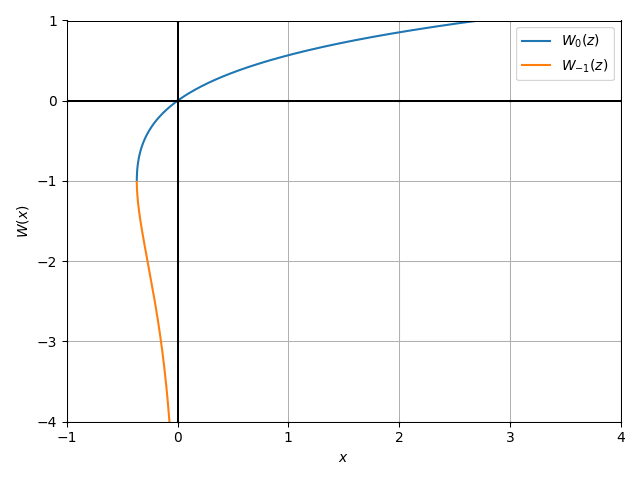
\includegraphics[width=.6\textwidth]{resources/lambertw.png}
    \caption{Les deux branches réelles de $W(x)$ lorsque $x$ est réel}
    \label{fig:lambertw}
  \end{center}
\end{figure}

\subsection{Évaluation de la fonction $W$}

Le fait qu'il n'existe pas de fonctions mathématiques élémentaires donnant explicitement $W(z)$ est remédié par l'existence de plusieurs \textit{algorithmes de recherche des zéros} permettant le calcul de les valeurs de n'importe quelle branche de la fonction $W$. Dans notre cas spécifique, la bibliothèque scientifique \textit{scipy} de Python fournit une fonction W implémentée par l'itération de Halley qui est un exemple d'une méthode de classe "Householder". La méthode de Halley a été appliquée à la fonction $W$  par Corless et al. \cite{Corless1996} donnant:
\begin{equation}
  \label{eq:halley}
  w_{j+1} = w_j - \frac{w_j e^{w_j} - z}{e^{w_j}(w_j + 1) - \frac{(w_j + 2)(w_j e^{w_j} - z)}{2w_j + 2}}
\end{equation}

Un exemple basique de l'utilisation de cette méthode en Python est le suivant:

\begin{python}[basicstyle=\tiny]
import numpy as np 
from scipy.special import lambertw #la bibliotheque scipy fourni la fonction W

z = np.linspace(-1/np.e, 3, 1000) # evaluons W entre -1/e et 3
w0 = lambertw(z, 0)
\end{python}

\subsection{Résolution de modèles simple et double diode par la fonction W}
De la définition de la fonction W, la solution d'une équation $xe^x = a$ est $x = W(a)$. En effectuent des manipulations algébriques élémentaires sur le modèle simple diode (equation \ref{eq:single}), Jain et Kapoor ont montré que l'expression explicite du courant en fonction des paramètres et de la tension est:
\begin{equation}
  \label{eq:lambertwsingle}
  I = \frac{R_{sh}(I_0 + I_{PV}) - V}{R_s + R_{sh}} - \frac{W\left(\frac{R_s I_0 R_{sh}}{a V_{th}(R_s + R_{sh})}e^{\left(\frac{R_{sh}(R_s I_{PV} + R_s I_0 + V)}{a V_{th} (R_s + R_{sh})}\right)}\right)aV_{th}}{R_s}
\end{equation}
On remarque bien que le second membre ne contient nul part un terme de courant $I$. Il faut noter aussi que le terme de la fonction $W$ est sous risque d'un dépassement et de retourner de valeurs infinies. Pour des raisons de stabilité numérique on utilise la notion de \textit{Conductance Shunt}: $C_{sh} = \frac{1}{R_{sh}}$ car cette résistance prend souvent de valeurs $\gg 1$ ce qui entraîne un risque de divergence des calculs.

Le modèle double diodes (équation \ref{eq:doublediode}) contient un terme exponentiel pour chaque diode. De la même manière que Jain et Kapoor on retrouve explicitement l'expression du courant avec deux termes de la fonction $W$ (equation \ref{eq:lambertwdouble}).
\begin{equation}
  \label{eq:lambertwdouble}
  \begin{split}
    I &= \frac{R_{sh} (I_{01} + I_{02} + I_{PV}) - V}{R_s + R_{sh}}\\ 
    &- \frac{a_1}{2 R_s} W\left( \frac{R_s R_{sh}(I_{01} + I_{02})}{a_1 (R_s + R_{sh})}e^{\left(\frac{R_{sh}(R_s I_{PV} + R_s I_{01} + R_s I_{02} + V)}{a_1 (R_s + R_{sh})}\right)}\right)\\ 
    &- \frac{a_2}{2 R_s} W\left( \frac{R_s R_{sh}(I_{01} + I_{02})}{a_1 (R_s + R_{sh})}e^{\left(\frac{R_{sh}(R_s I_{PV} + R_s I_{01} + R_s I_{02} + V)}{a_2 (R_s + R_{sh})}\right)}\right)
  \end{split}
\end{equation}

\section{Résultats}

\section{Conclusion}
